\chapter{Radio Physics}\label{ch:radio-physics}
%\bibtodo{from original report}
The goal of this chapter is to be able to estimate the probability, based on the topology of a wireless
network, of how likely it is that packet loss will happen during transmission between two nodes.

%\autoref{sec:linkmodel} presents the method for simulating the link model in a \gls{manet}, \autoref{sec:pep}
%presents the method for computing the packet loss probability during a transmission, and
%\autoref{sec:optimization} proposes two ways for optimising the computational time required to compute the
%link model.

\begin{figure}[ht]
    \centering
    \includegraphics[width=.65\textwidth]{figures/manet_with_terrain.png}
    \caption{A wireless network topology.}
    \label{figure:manetwithter}
\end{figure}

\autoref{figure:manetwithter} shows a sample wireless network topology for a \acrfull{manet}. The network
consists of mobile devices (nodes), and the communication between these (links). Nodes are
\doublequote{linked} with other nodes when they can communicate wirelessly. Wireless communication relies on
the transmission and reception of electromagnetic waves~\cite[p.~10]{paper:linkmodel} (radio signals), and the
strength, or quality, of a wireless link, is described by the signal loss occurring when propagating the
signal from transmitter to receiver, and is measured by the \gls{rssi} (a negative value, where a value close
to 0 is better). In \cite{paper:linkmodel}, the term \gls{pathloss} is used to describe this signal loss and
is determined in part by the physical distance between transmitter and receiver, but also by physical objects
and terrain, like buildings or forests. A major consideration for mobile networks is that the topology is
dynamic. Nodes move around, causing links to disappear, or new links to appear, thus changing the topology of
the network. \autoref{sec:visualiser} introduces the Visualiser and presents the proposed extensions.
\autoref{sec:hardwarephysics} introduces a series radio specific terms we use throughout the thesis.
\autoref{sec:reachi-experiments} presents the link \gls{pathloss} model from \cite{paper:linkmodel}, and
\autoref{sec:linkmodel} introduces an alternative \gls{pathloss} model based on building footprints between
nodes in a links, by using OpenStreetMap map tiles. Finally, \autoref{sec:radiomodel} presents the method for
simulating packet loss and transmission interference.

%\autoref{sec:linkmodel} will elaborate
%further on the \gls{pathloss} of a link, as well as present a method for simulating the \gls{pathloss} for a
%mobile network topology. 

\section{Visualiser Tool}\label{sec:visualiser}
The Visualiser is a tool written in Python and JavaScript, created by Peter Gjøl Jensen. The tool was created
to aid in visualisation of \gls{manet} topologies, and works by importing a log file with \acrshort{gps}
coordinates and timestamps for a series of nodes. Using the tool, it is possible to visualise the position and
movement for all nodes in a network. A snippet of a \acrshort{gps} log can be seen below. Each line consists
of the identifier of the node, the latitude and longitude coordinates for the node, and the timestamp for the
coordinates in milliseconds.
%
\begin{verbatim}
#id,lat,lon,timestamp
64,14.629879,121.096137,158980000.000000
64,14.629874,121.096132,159000000.000000
64,14.629878,121.096128,159020000.000000
64,14.629890,121.096143,159040000.000000
64,14.629892,121.096142,159060000.000000
64,14.629896,121.096141,159080000.000000
64,14.629893,121.096164,159100000.000000
64,14.629947,121.096083,159120000.000000
64,14.630107,121.095976,159140000.000000
64,14.630283,121.095885,159160000.000000
64,14.630525,121.095786,159180000.000000
\end{verbatim}

\autoref{figure:gpslogvisualised} in \autoref{app:visualiser:screens} shows a screen-shot from the Visualiser,
with a \acrshort{gps} log loaded. When a \acrshort{gps} log is loaded, the Visualiser can be started by
pressing the \doublequote{Play} button, or the \doublequote{space} key. The speed of the visualisation can be
controlled with the \doublequote{Speed} slider in the bottom, and the current time of the visualisation can
be controlled with the \doublequote{Time} slider. 

\subsection{Extensions}
We propose three extension to the visualiser tool. The first is to visualise the link between nodes using an
annotated version of the \acrshort{gps} log, where each line is annotated with the \gls{rssi} of a link
between nodes in the log, as shown below. In the annotated log, each link for a given node, to another node,
is annotated, after the timestamp, with the identifier of the other node, and the \gls{rssi} between them.
\autoref{figure:gpslogrssivisualised} in \autoref{app:visualiser:screens} show an example of a very connected
network where links between nodes are visualised by a colour gradient, where a link with a yellow colour has a
better \gls{rssi} than a link with a red colour. It is possible to print the \gls{rssi} value for the links as
well.
%
\begin{verbatim}
#id,lat,lon,timestamp,id1,rssi1,id2,rssi2,id3,rssi3, ...
65,14.630107,121.096749,157820000.000000,67,-56,69,-70,71,-13, ...
65,14.630129,121.096905,157840000.000000,67,-58,69,-61,73,-65, ...
65,14.630189,121.097116,157860000.000000,67,-55,69,-54,73,-71, ...
65,14.630318,121.097294,157880000.000000,67,-65,69,-66,71,-13, ...
65,14.630330,121.097545,157900000.000000,67,-79,69,-48,73,-79, ...
65,14.630358,121.097725,157920000.000000,67,-85,69,-66,71,-28, ...
65,14.630243,121.097900,157940000.000000,69,-84,71,-35,83,-67, ...
65,14.630082,121.098037,157960000.000000,71,-45,83,-70,89,-43, ...
65,14.629960,121.098165,157980000.000000,71,-20,83,-75,89,-38, ...
65,14.629729,121.098192,158000000.000000,83,-81,89,-42,97,-80, ...
\end{verbatim}

The second extension is to be able to replay the communication between nodes when simulating a protocol. This
log is generated by the Coordinator (introduced in \autoref{sec:coordinator}), and a line is added whenever a
packet is either dropped or received during a transmission. Each line states whether the packet was received
or dropped, the identifier of the transmitter and receiver, the number of bytes sent, the \gls{rssi} for the
transmission, the probability for packet error, that decided whether the packet was dropped or not, the
interfering power and the number of interfering transmitters (if any), and finally, the start and end time of
the transmission. With this log, it is possible to visualise any transmissions by drawing a unidirectional
arrow from the transmitter to the receiver, within the time interval of the transmission.
%
\begin{verbatim}
#received,tx_id,rx_id,bytes,rssi,pep,int_power,ints,tx_start,tx_end
recv,1,2,2,-102.419,5.74662e-05,0,0,2233,2692
recv,1,5,2,-102.419,5.7577e-05,0,0,2233,2692
drop,1,6,2,-110.697,0.494838,0,0,2233,2692
drop,1,6,24,-110.697,0.999724,0,0,12692,18209
recv,1,5,24,-102.419,0.000690706,0,0,12692,18209
recv,1,2,24,-102.419,0.000689376,0,0,12692,18209
recv,1,2,2,-102.419,5.74662e-05,0,0,32002048,32002507
recv,1,5,24,-102.419,0.000690706,0,0,32012507,32018024
recv,1,2,24,-102.419,0.000689376,0,0,32012507,32018024
\end{verbatim}

The third, and final, extension is to replay state changes of a protocol. When simulating a protocol like the
\gls{lmac} protocol (introduced in \autoref{sec:lmacc}), where each node proceeds through a number of states,
we log each of the state changes, as shown below, and can replay these state changes in the Visualiser.
%
\begin{verbatim}
#timestamp,id,state
0,10,i
0,1,i
0,9,i
800.009,1,0
800.002,2,w
5600,2,d
800.002,5,w
4800,5,d
5600.01,5,5
6400.01,2,6
6400,6,w
8800,6,d
\end{verbatim}

A visualised example of the second and third extension for an execution of the \gls{lmac} protocol can be
found at \autoref{fig:lmac-visualisation} in \autoref{sec:lmacc}. \medbreak

%\todo[inline]{introduce}
%\todo[inline]{why}
%\todo[inline]{screenshots and short description of what it can do}

The complete source code for the Visualiser tool can be found on GitHub:

{\small \url{https://github.com/Joklost/manet-simulations/tree/master/tools/visualiser}}
%
\section{Radio Hardware}\label{sec:hardwarephysics}
\todo[inline]{rssi, transmission time (baudrate), reachi constants}
\todo[inline]{hardware section with transmission power, pathloss, rssi and so on rssi = txpower-pathloss}

Transmission power is 

\gls{rssi} is the perceived signal strength of a link.

\gls{pathloss} is the signal loss inflicted by the propagation of an electromagnetic wave from transmitter to
receiver.


\autoref{eq:transmission-time} computes the amount of time required to transmit a packet, in microseconds,
based on the \gls{baudrate} $f_s$ and the size of a packet in bytes. For a packet where $|\mathit{packet}| = 20$
bytes would take $\mathit{transmissiontime}(|\mathit{packet}|) = 4597$ microseconds, with \gls{baudrate} $f_s =
34800$ Hz.
%
\begin{eq}\label{eq:transmission-time}
    \mathit{transmissiontime}(\mathit{packetsize}) = \frac{1000000}{f_s} \cdot \left( \mathit{packetsize} \cdot 8
    \right)
\end{eq}

\section{Link Path Loss}\label{sec:reachi-experiments}
In this section, we present the method for simulating link \gls{pathloss} from \cite{paper:linkmodel}, as well
as why the model does not work for our needs. For our own simulations, we want to simulate the performance of
nodes in a \gls{manet}. The performance is, however, heavily dependent on network conditions and the
capabilities of the technology~\cite[p.~10]{paper:linkmodel}. The author of \cite{paper:linkmodel} presents
methods for evaluating the performance of a wireless network, and proceeds to introduce methods for simulating
\gls{pathloss} on a multi-link model, based on real-world performance measurements. \medbreak

The author of \cite{paper:linkmodel} describes the \gls{pathloss} of a link to be the sum of two parts: A
deterministic distance dependent part, that describes the mean signal attenuation at any given link distance,
and a stochastic shadow fading part, which is the \gls{pathloss} caused by terrain, buildings, vegetation and
cars. With this \gls{pathloss} it is possible to simulate the \gls{rssi} on a given link, by subtracting the
\gls{pathloss} from the transmission power of the simulated radio.
%
\begin{eq}\label{eq:ld}
    \mathit{pl}_d(l) = 55 \log_{10}(d(l)) - 18.8
\end{eq}

The distance dependent \gls{pathloss} is computed using the $\mathit{pl}_d(l)$ function shown in
\autoref{eq:ld}~\cite[p.~25]{paper:linkmodel}, where the function $d(l)$ denotes the distance of a link in
meters. Computing the shadow fading \gls{pathloss}, on the other hand, is not as trivial. The shadow fading
part of the \gls{pathloss} is based on the correlation between angles of link pairs sharing a common nodes,
and bears a significant practical limitation in the sense that the shadow fading part depends on a Cholesky
factorisation with a computational complexity of $O(N^6)$~\cite[p.~31]{paper:linkmodel}, where $N$ is the
total number of nodes in the network. \medbreak

Through personal communication with the author of \cite{paper:linkmodel}, we received access to logs from
field experiments for the Reachi project. These field experiments were conducted in different locations with
an early prototype of the Reachi device. The logs contain \gls{gps} coordinates, as well as \gls{rssi}
information for detected neighbours of each node. Examining these logs has shown discrepancies between the
\gls{pathloss} model from \cite{paper:linkmodel} and the measured \gls{rssi}.
\autoref{plot:reachi-experiments:measurements-vs-ld} plots samples drawn from the $\mathit{pl}_d(l)$ function
and measurements from a log containing field measurements from an experiment in Marikina, in the Phillippines.
Since the log contained a total of 17761 links, the measurements are summarised based on the distance of the
link, and each link was sorted into distance buckets with 20 meter intervals. The average \gls{rssi} for all
links in a bucket is plotted in \autoref{plot:reachi-experiments:measurements-vs-ld}. The plot shows that the
\gls{rssi} computed with the distance dependent \gls{pathloss} does not fit with the measured \gls{rssi}.
\medbreak

As mentioned earlier, the shadow fading \gls{pathloss} is based on the correlation between angles of link
pairs that share a common node. An assumption for this is that link pairs with a high correlation, where the
angle between them is low, will have close to the same shadow fading~\cite{paper:linkmodel}. However, this
does not seem to be the case. \autoref{plot:reachi-experiments:avg-rssi-angle-phili-rude} show a plot where we
compare the Marikina log from earlier, with another field experiment log from Rude Skov. For both logs, pairs
of links sharing a common node were sorted, based on the angle between them, into buckets of 5 \degree
intervals, and we computed the average \gls{rssi} for these buckets, after removing the distance dependent
\gls{pathloss}. This means that only the shadow fading part of the \gls{pathloss} is included in the
\gls{rssi} plotted in \autoref{plot:reachi-experiments:avg-rssi-angle-phili-rude}. Under the assumption that a
highly correlated link pairs should result in less shadow fading \gls{pathloss}, the traces on
\autoref{plot:reachi-experiments:avg-rssi-angle-phili-rude} should increase gradually as the angle increases.
This is not the case. \medbreak

Because of this, and the fact that computing the shadow fading path loss is not feasible for a very large
number of nodes, we instead propose our own model for approximating the shadow fading \gls{pathloss}.

%As mentioned above, the angle based approach relies on the assumption that link pairs with a high correlation,
%i.e. low angle between them, will have close to the same shadow fading. We have however not been able to
%produce reliable proof that the assumption is correct. To produce proof, the Marikina and Rude skov log was
%used. 

%For both logs, link pairs were created and sorted based on their angle into separate bucekts of
%5$\degree$ intervals. The average \gls{rssi} for each bucket was then computed. Before computing the average
%\gls{rssi}, the distance dependent part $l_d$ was removed from the links \gls{rssi} measurement, to isolate
%the stochastic part. The resulting data can be seen plotted on
%\autoref{plot:reachi-experiments:avg-rssi-angle-phili-rude}. Under the previous assumption that a high
%correlation gives smaller stochastic path loss, then the traces on
%\autoref{plot:reachi-experiments:avg-rssi-angle-phili-rude} should increase gradually as the angle increases.
%Clearly the measurements does increase as the angle increase, but the increaes are not steady but rather vary
%greatly. Too greatly to say that with certainty that the assumption holds on the received logs.

\begin{figure}[H]
    \centering
    \begin{tikzpicture}
        \begin{axis}[
                height=10.5cm, width=0.95\textwidth,
                ylabel={RSSI},
                xlabel={Distance in meters},
                axis lines*=left,
                xmin=0, xmax=750,
                enlargelimits=false,
                ymin=-120, ymax=-20,
                xtick={0, 50, 100, 150, 200, 250, 300, 350, 400, 450, 500, 550, 600, 650, 700, 750},
                ymajorgrids=true,
                xmajorgrids=true,
                grid style=dashed,
                restrict y to domain=-120:-20,
                samples=600
            ]

            \addplot[very thick, solid, cyan, mark=*] coordinates {(20, -28.32345013477089) (40, -44.85830258302583) (60, -52.77323717948718) (80, -60.21201657458563) (100, -66.47435897435898) (120, -69.68905472636816) (140, -71.5976496922216) (160, -73.7866473149492) (180, -75.53428571428572) (200, -76.89289392378991) (220, -77.88135593220339) (240, -77.8035019455253) (260, -77.36784140969164) (280, -77.14030612244898) (300, -77.75299760191847) (320, -79.71686746987952) (340, -79.15481171548117) (360, -79.90728476821192) (380, -81.30909090909091) (400, -81.79746835443038) (420, -81.52272727272727) (440, -79.2) (460, -79.42105263157895) (480, -79.4375) (500, -79.0) (520, -77.91666666666667) (540, -83.0) (560, -81.27272727272727) (580, -83.57142857142857) (600, -86.0) (620, -83.4) (640, -86.5) (660, -81.42857142857143) (680, -79.0) (700, -82.71428571428571) (740, -77.0)};
            \addlegendentry{Marikina field measurements};

            \addplot[domain=0:740, very thick, solid, red] {26 - ld(x)};
            \addlegendentry{Computed \gls{rssi}};
        \end{axis}
    \end{tikzpicture}
    \caption{Average RSSI pr. distance bucket.}\label{plot:reachi-experiments:measurements-vs-ld}
\end{figure}

\begin{figure}[H]
    \centering
    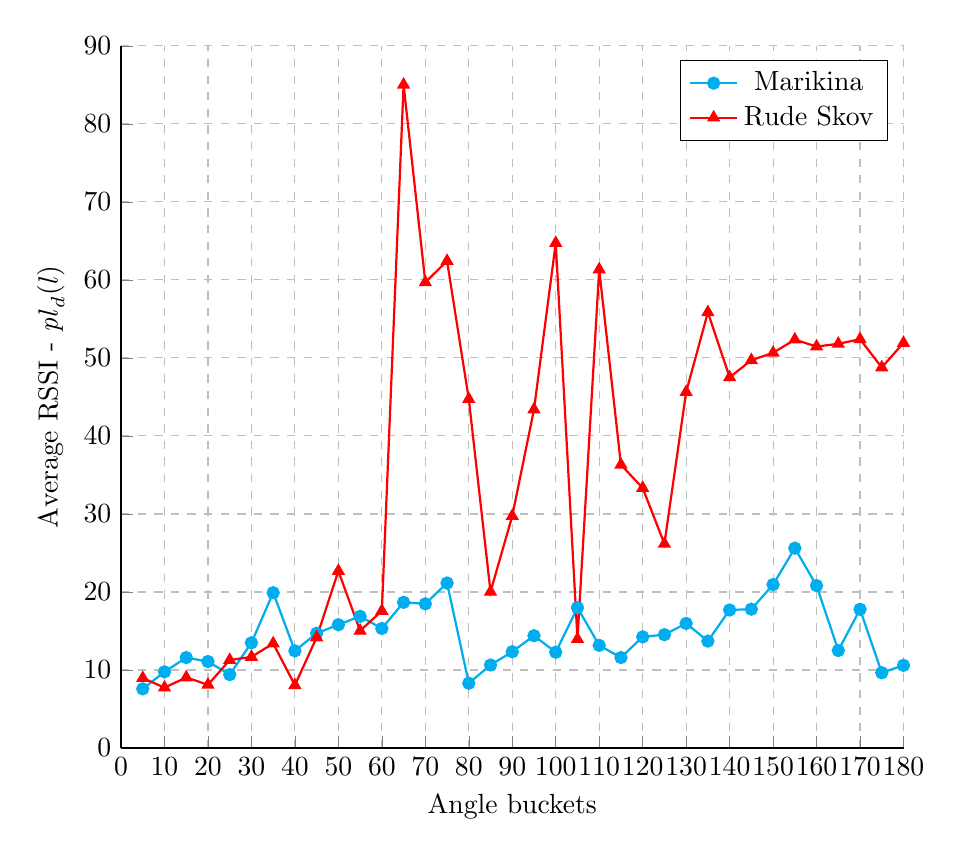
\begin{tikzpicture}
        \begin{axis}[
                height=10.5cm, width=0.95\textwidth,
                ylabel={Average RSSI - $\mathit{pl}_d(l)$},
                xlabel={Angle buckets},
                axis lines*=left,
                xmin=0, xmax=180,
                xtick={0, 10, 20, 30, 40, 50, 60, 70, 80, 90, 100, 110, 120, 130, 140, 150, 160,170,180},
                enlargelimits=false,
                ymin=0, ymax=90,
                ymajorgrids=true,
                xmajorgrids=true,
                grid style=dashed
            ]

            \addplot[thick, solid, cyan, mark=*] coordinates {(5,7.581215097994852)(10,9.763581254686114)(15,11.59234807189617)(20,11.084399582147876)(25,9.411670936293284)(30,13.486232393853125)(35,19.91110051641767)(40,12.453590557884946)(45,14.70313120243339)(50,15.804939314638208)(55,16.87697870999425)(60,15.320902904198922)(65,18.673392004683087)(70,18.48508963612783)(75,21.147550183881993)(80,8.302184073487094)(85,10.641508684206432)(90,12.343183048128944)(95,14.396643466792797)(100,12.27504884861337)(105,17.994872329043496)(110,13.156645245862158)(115,11.595967499573286)(120,14.245146945189493)(125,14.528392002600814)(130,15.96981736460891)(135,13.70427190114752)(140,17.692009757218077)(145,17.79486440192431)(150,20.947579654378668)(155,25.611175147469265)(160,20.819124899373364)(165,12.495568407794714)(170,17.784042978338544)(175,9.646875797269503)(180,10.597197732034614)};
            \addlegendentry{Marikina};


            \addplot[thick, solid, red, mark=triangle*] coordinates {(5,8.968175725354994)(10,7.741408675352775)(15,9.042742837449076)(20,8.108954051047618)(25,11.273321343260399)(30,11.67692967914715)(35,13.401460743255232)(40,8.053793318539391)(45,14.17474549040368)(50,22.68855220716477)(55,15.026896145186285)(60,17.5755161176863)(65,85.01233086400362)(70,59.69038212814202)(75,62.41948703096457)(80,44.72712810089782)(85,20.029080610052482)(90,29.737954905927445)(95,43.39235466255519)(100,64.720015835849)(105,13.965589072181558)(110,61.334883149884675)(115,36.30455538419785)(120,33.32223486902817)(125,26.172354285886417)(130,45.62355888699502)(135,55.8474401182669)(140,47.511612928722954)(145,49.70429537245245)(150,50.649080550831435)(155,52.34402139529124)(160,51.45218633523966)(165,51.805898996936115)(170,52.39131328924595)(175,48.78102582759046)(180,51.91529108595685)};
            \addlegendentry{Rude Skov};
        \end{axis}
    \end{tikzpicture}
    \caption{Average \gls{rssi} per angle bucket without distance dependent \gls{pathloss}.}
    \label{plot:reachi-experiments:avg-rssi-angle-phili-rude}
\end{figure}
\section{Link Modelling}\label{sec:linkmodel}
In this section, we propose a method for modelling and computing link \gls{pathloss} using building footprints
between nodes of a link, on OpenStreetMap map tiles obtained through the Mapbox Maps Service
API~\cite{website:mapbox}. The model computes the \gls{pathloss} based on the distance of the link and the
percentage of that distance that is in a building. Buildings and other environmental obstructions, which is
part of the shadow fading \gls{pathloss} from \cite{paper:linkmodel}, should cause a higher \gls{pathloss}, as
it is harder for the radio signal to propagate through buildings. \medbreak

The main idea is to generate a map of the area that contains nodes of a link as an image, and when computing
the \gls{pathloss} of that link, count the percentage of all pixels in a straight line between the nodes in a
link that are considered buildings on the map. The pseudo code description of this can be seen in
\autoref{algo:linkmodel:compute-building-percentage}.

%In this section, our own Linkmodel will be described.

%\subsection{Computing path loss}
%To facilitate to the problems discussed in \autoref{sec:reachi-experiments}, we have devised our own linkmodel
%to compute path loss. 
%Our model computes path loss based on the distance of the link and the percentage of
%that distance that is in a building. Building and other obstructions in the environment cause more severe path
%loss, and as such should be considered to punish the signal more. Our model limits to only buildings. 

%The idea
%is to generate a map of the area that the nodes are located in as an image, then when computing the path loss
%of a link, look up the colour of all pixels in a straight line between the nodes  of link and count how many
%is a building. This gives a percentage for how much of the distance is covered by buildings. An pseudo code
%implementation of the computation can be seen on \autoref{algo:linkmodel:compute-building-percentage}.

\begin{algorithm}[ht]
    \DontPrintSemicolon
    \KwIn{$(x_1, y_1), (x_2, y_2)$}
    \KwOut{Percentage building between points.}
    \SetKwFunction{FLoSModelCompute}{CompBuildingPct}
    \SetKwProg{Fn}{Function}{}{}

    \Fn{\FLoSModelCompute{$(x_1, y_1), (x_2, y_2)$}}{
        %$(n_1,\ n_2) \leftarrow \mathit{nodes}(l)$\;
        %$(x_1,\ y_1) \leftarrow$ compute position for $n_1$\;
        %$(x_2,\ y_2) \leftarrow$ compute position for $n_2$\;
        %\;
        $\mathit{pixels} \leftarrow 0$\;
        $\mathit{buildings} \leftarrow 0$\;
        \While{$\lambda \in \{0 \dots 1\}$}{
            $(x,\ y) \leftarrow \lambda \cdot (x_1,\ y_1) + (1 - \lambda)\cdot(x_2,y_2)$\;
            \If{position ($x$, $y$) is a building}{
                $\mathit{buildings} \leftarrow \mathit{buildings} + 1$\;
            }
            $\mathit{pixels} \leftarrow \mathit{pixels} + 1$\;
        }

        \KwRet $\frac{\mathit{buildings}}{\mathit{pixels}}$\;
    }
    \caption{The CompBuildingPct function.}
    \label{algo:linkmodel:compute-building-percentage}
\end{algorithm}

To compute the total \gls{pathloss}, we first define two functions: $\mathit{cvpl}(l)$ (\gls{cvpl}) and
$\mathit{bopl}(l)$ (\gls{bopl}). Both functions compute the distance-dependent \gls{pathloss}, similarly to
the $\mathit{pl}_d$ function from \autoref{sec:reachi-experiments}, but rather than computing the total
distance based \gls{pathloss}, we need to define a similar function for the distance with a clear view, and a
similar function to the distance where buildings obstruct the signal. To do this, we define this as an
optimisation problem, where we want to find the optimal constants for the two functions, by minimising the
difference between the computed \gls{rssi} and the measured \gls{rssi} for a set of links $L$. The
$\mathit{compRSSI}(l) = \mathit{tx}_\mathit{power} - (\alpha \cdot (\ln(d(l)) / \ln(\delta)) + \beta)$
function denotes the computed \gls{rssi} for a link with the chosen values for $\alpha$, $\beta$, and
$\delta$.
\medbreak

The problem is defined as follows:

\begin{itemize}
    \item Input: A set of links $L$.
    \item Output: Optimal values for $\alpha, \beta, \delta$.
    \item Goal: Minimise the $\mathit{score}(\alpha, \beta, \delta)$ function:

          $\mathit{score}(\alpha, \beta, \delta) = \mathlarger{\sum}\limits_{l \in L} (\mathit{compRSSI}(l) - \mathit{measuredRSSI}(l))^2$
\end{itemize}

\subsection{Greedy Approach}
To solve the optimisation problem, we have chosen a greedy approach. First, to compute the optimal values for
the $\mathit{cvpl}(l)$ function, we compile a set of links $L$, where the computed building percentage is
below 5 \%, and for the $\mathit{bopl}(l)$ function, we compile a set of links $L$ where the computed building
percentage is above 80 \%. Ideally, we would like for the building percentage to be close to 100 \%, but the
number of links in the Marikina log with more than 95 \% of buildings is very low. With these sets, we attempted
to find the optimal values for $\alpha$, $\beta$, and $\delta$ by going through $\alpha, \beta \in \{-100,
\dots, 100\}$ with increments of $0.5$, and $\delta \in \{2, \dots, 100\}$ with increments of $1$. This
resulted in the following values for the $\mathit{cvpl}(l)$ and $\mathit{bopl}(l)$ functions:
%
\begin{eq} 
    \mathit{cvpl}(l) = 48.5 \cdot (\ln{(d(l))} / \ln{(77)}) + 37.5 
\end{eq}

\begin{eq} 
    \mathit{bopl}(l) = 67 \cdot (\ln{(d(l))} / \ln{(57))} + 11.5 
\end{eq}


%To solve the optimisation problem, brute forcing will be utilised because of time restrictions. The set of
%links $L$, consisted of links with a computed building percentage below five percent or above 80\% was
%collected from the Marikina log into their separate collections. The Marikina log was used because the
%experiment was conducted in a city, resulting in links with varying building percentages. For both
%collections the links were further sorted based on distance of the links, with 20 meter intervals i.e. links
%with distances between 20 meters and 40 meters was sorted together. The average \gls{rssi} for each
%separation was then computed. Links with building percentage above 80\% was used for $\mathit{bopl}$ and
%links below 5 percent for $\mathit{cvpl}$. The parameters $\alpha,\ \beta \in \{-100 \dots 100\}$ with $0.5$
%increments and $\delta\ \in \{2 \dots 100\}$ with $1$ increments. The result was the following functions:
%\begin{eq} \mathit{cvpl}(l) = 48.5 \cdot (\ln{(d(l))} / \ln{(77)}) + 37.5 \end{eq}
%
%\begin{eq} \mathit{bopl}(l) = 67 \cdot (\ln{(d(l))} / \ln{(57))} + 11.5 \end{eq}


%We define two functions, $\mathit{cvpl}(l)$ and $\mathit{bopl}(l)$. Both functions compute path
%loss based on distance. \gls{cvpl} computes path loss for distances with zero percent building, while
%\gls{bopl} computes path loss for 100\% building. When computing the path loss both functions will be used, in
%the following equation:
%\todo[inline]{make me prettier}

%\todo[inline]{finish block}


%Finding the optimal constants for $\mathit{cvpl}$ and $\mathit{bopl}$ can defined as an optimisation problem.
%A set of links $L$ must be provided. The goal is to compute the difference from the computed \gls{rssi} to the
%measurements for all links in $L$.
%\medbreak

%The problem is defined as follows:
%\begin{itemize}
%    \item Input: A set of link $L$.
%    \item Output: Optimal parameters for $\alpha,\ \beta,\ \delta$.
%    \item Goal: Minimise the score function:\smallbreak
%    $\mathit{compRSSI}(l)= \alpha \cdot (log_\delta(d(l))) + \beta$\smallbreak
%    $\mathit{score}(\alpha, \beta, \delta) = \sum\limits_{l\ \in\ L} (\mathit{compRSSI}(l) - \mathit{measuredRSSI}(l))^2$
%
%\end{itemize}

With these two functions defined, we can compute the total \gls{pathloss} for a link. The function
$p(l)$ denotes the points for the links, as required by the input to the CompBuildingPct function.
%
\begin{eq}\label{eq:pl} %%% REMEMBER %%%
    \mathit{pl}(l) = (\mathit{cvpl}(l) \cdot (1 - \text{CompBuildingPct}(p(l)))) + (\mathit{bopl}(l) \cdot \text{CompBuildingPct}(p(l)))
\end{eq}

Finally, with the $\mathit{pl}(l)$ function, we can compute the \gls{rssi} for the link $l$: 
%
\begin{eq}\label{eq:plrssi}
    \mathit{RSSI}_{\mathit{dBm}}(l) = \mathit{tx}_\mathit{power} - \mathit{pl}(l)
\end{eq}

\subsection{Evaluation}

The functions $\mathit{cvpl}(l)$ and $\mathit{bopl}(l)$ have been plotted
on \autoref{plot:reachi-experiments:cvpl-vs-bopl}. $\mathit{bopl}$ do result in greater \gls{pathloss}, however,
the plot also reveals that up to 100 meters, $\mathit{bopl}(l)$ compute a better \gls{rssi} compared to
$\mathit{cvpl}(l)$. To further examine this, each function has been plotted with their training set.
$\mathit{cvpl}(l)$ on \autoref{plot:reachi-experiments:marikina-log-below-5-pct} and $\mathit{bopl}(l)$ can be
seen in \autoref{plot:reachi-experiments:marikina-log-above-80-pct}.

\begin{figure}[H]
    \centering
    \begin{tikzpicture}
        \begin{axis}[
                height=10cm, width=0.95\textwidth,
                ylabel={RSSI},
                xlabel={Distance in meters},
                axis lines*=left,
                xmin=0, xmax=750,
                enlargelimits=false,
                ymajorgrids=true,
                xmajorgrids=true,
                grid style=dashed,
                restrict y to domain=-120:0,
                samples=700
            ]

            \addplot[domain=0:1000, very thick, solid, cyan] {26 - bopl(x)};
            \addlegendentry{\gls{bopl}};

            \addplot[domain=0:1000, very thick, dashed, red] {26 - cvpl(x)};
            \addlegendentry{\gls{cvpl}};
        \end{axis}
    \end{tikzpicture}
    \caption{Plot showing samples drawn from \gls{cvpl} and \gls{bopl}}
    \label{plot:reachi-experiments:cvpl-vs-bopl}
\end{figure}

\begin{figure}[H]
    \centering
    \begin{tikzpicture}
        \begin{axis}[
                title={score: 501.4932, links: 13481, score/link: 0.0372},
                height=10cm, width=0.95\textwidth,
                ylabel={RSSI},
                xlabel={Distance in meters},
                axis lines*=left,
                xmin=0, xmax=750,
                enlargelimits=false,
                ymin=-90, ymax=-30,
                xtick={0, 50, 100, 150, 200, 250, 300, 350, 400, 450, 500, 550, 600, 650, 700, 750},
                ymajorgrids=true,
                xmajorgrids=true,
                grid style=dashed,
                samples=700
            ]

            \addplot[very thick, solid, cyan, mark=*] coordinates {(20, -36.01344537815126) (40, -48.361111111111114) (60, -54.93279022403259) (80, -62.40816326530612) (100, -68.14871794871794) (120, -60.85954712362301) (140, -71.69568452380952) (160, -74.36896551724138) (180, -73.93817204301075) (200, -75.09929078014184) (220, -73.38403041825094) (240, -75.43994413407822) (260, -77.69102990033223) (280, -77.31512605042016) (300, -75.7751937984496) (320, -78.60714285714286) (340, -78.38524590163935) (360, -78.52459016393442) (380, -77.34285714285714) (400, -80.96153846153847) (420, -81.03571428571429) (440, -80.41379310344827) (460, -74.18181818181819) (480, -79.9090909090909) (500, -79.75) (520, -77.56521739130434) (540, -81.23076923076923) (560, -78.9) (580, -85.0) (620, -82.5) (640, -82.33333333333333) (660, -82.4) (680, -77.5) (700, -85.4) (740, -77.0)};
            \addlegendentry{Marikina field measurements}


            \addplot[domain=0:740, very thick, solid, red] {26 - cvpl(x)};
            \addlegendentry{\gls{cvpl}};
        \end{axis}
    \end{tikzpicture}
    \caption{Field measurements with building percentage below 5 \%.}
    \label{plot:reachi-experiments:marikina-log-below-5-pct}
\end{figure}

\begin{figure}[H]
    \centering
    \begin{tikzpicture}
        \begin{axis}[
                title={score: 350.6854, links: 377, score/link: 0.9302},
                height=10cm, width=0.95\textwidth,
                ylabel={RSSI},
                xlabel={Distance in meters},
                axis lines*=left,
                xmin=0, xmax=380,
                enlargelimits=false,
                ymin=-90, ymax=-30,
                ymajorgrids=true,
                xmajorgrids=true,
                grid style=dashed,
                samples=400
            ]

            \addplot[very thick, solid, cyan, mark=*] coordinates {(20, -32.56521739130435) (40, -50.607142857142854) (60, -52.15384615384615) (80, -64.85714285714286) (100, -49.5) (120, -65.76623376623377) (140, -69.38888888888889) (160, -72.05714285714286) (180, -69.3125) (200, -78.83333333333333) (220, -76.84) (240, -75.75) (260, -80.91666666666667) (280, -72.88888888888889) (300, -78.95238095238095) (320, -76.44444444444444) (340, -82.75) (380, -87.0)};
            \addlegendentry{Marikina field measurements};

            \addplot[domain=0:380, very thick, solid, red] {26 - bopl(x)};
            \addlegendentry{\gls{bopl}};
        \end{axis}
    \end{tikzpicture}
    \caption{Field measurements with building percentage above 80 \%.}
    \label{plot:reachi-experiments:marikina-log-above-80-pct}
\end{figure}

With the optimal values for the $\mathit{cvpl}(l)$ function, the final score was 501.4932 for 13481 links with
less than 5 \% buildings. \autoref{plot:reachi-experiments:marikina-log-below-5-pct} shows how well this
function fits with the measured values. \smallbreak

For the $\mathit{bopl}(l)$ function, we got a final score of 350.6854 for 377 links with more than 80 \%
buildings. This is a very large difference compared to the 13481 links for the $\mathit{cvpl}(l)$, which means 
that we might experience lower precision for the $\mathit{bopl}(l)$ function.

%With the found optimal parameters for $\mathit{cvpl}$, the resulting was score was 501.4932 for 13481 links.
%The average score for a single link is then $0.0372 = 501.4932 / 13481$. We consider this as good score, and
%as can be seen on \autoref{plot:reachi-experiments:marikina-log-below-5-pct}, the function fits the
%measurements.\medbreak
%
%The $\mathit{bopl}$ however got worse result. The score per link was 0.9302 which is much larger compared to
%the score for $\mathit{cvpl}$. It is important to note that there was only 377 links in the training set for
%the $\mathit{bopl}$ function, which is vastly less compared to the 13481 links for the $\mathit{cvpl}$
%function. Another reason for the lower precision of $\mathit{bopl}$ is that the training set does not only
%consist of links with 100\% building, as we allowed for links with more than 80\%. This was however necessary
%as there was close to none links with 100\% building. Having a large set of links with 100\% building would
%result in higher precision.

Finally, a comparison of the computed \gls{rssi} values from \autoref{eq:plrssi} with the measurements from
the Marikina log is shown in \autoref{plot:reachi-experiments:marikina-log-vs-computed}. The plot shows that
the function is slightly off on the from about 75 meters to 300 meters, but compared to
\autoref{plot:reachi-experiments:measurements-vs-ld}, we do see an improvement.

\begin{figure}[ht]
    \centering
    \begin{subfigure}[b]{0.48\textwidth}
        \centering
        \qrcode[hyperlink]{https://youtu.be/vVqHzVThW34}
        \caption{Field measurements visualised.}
        \label{fig:field-measurements-visualised-qr}
    \end{subfigure}
    \hfill
    \begin{subfigure}[b]{0.48\textwidth}
        \centering
        \qrcode[hyperlink]{https://youtu.be/tZdhf6zcs2Y}
        \caption{Computed \gls{rssi} values visualised.}
        \label{fig:computed-values-visualised-qr}
    \end{subfigure}
    \caption{Marikina field measurements and computed \gls{rssi} values.}
    \label{fig:building-visualisation}
\end{figure}

\autoref{fig:building-visualisation} contains YouTube links to two visualisations, where 
\autoref{fig:field-measurements-visualised-qr} visualises the Marikina field measurements, and 
\autoref{fig:computed-values-visualised-qr} visualises the computed \gls{rssi} values. Both visualisations
highlight the same subset of the links, to make it easier to follow. \medbreak

The complete source code for the C++ implementation can be found on GitHub:

\url{https://github.com/Joklost/sims2}

\begin{figure}[H]
    \centering
    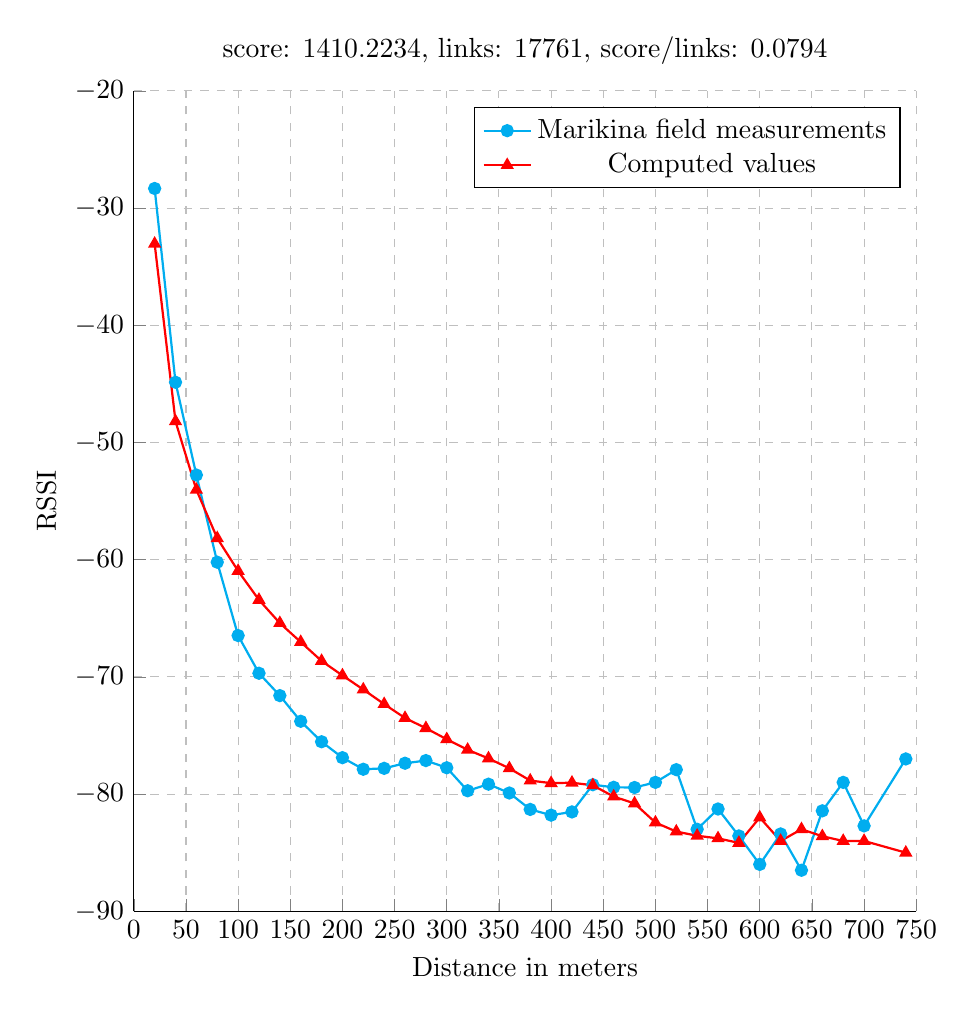
\begin{tikzpicture}
        \begin{axis}[
                title={score: 1410.2234, links: 17761, score/links: 0.0794},
                height=12cm, width=0.95\textwidth,
                ylabel={RSSI},
                xlabel={Distance in meters},
                axis lines*=left,
                xmin=0, xmax=750,
                enlargelimits=false,
                ymin=-90, ymax=-20,
                xtick={0, 50, 100, 150, 200, 250, 300, 350, 400, 450, 500, 550, 600, 650, 700, 750},
                ymajorgrids=true,
                xmajorgrids=true,
                grid style=dashed,
            ]

            \addplot[thick, solid, cyan, mark=*] coordinates {(20, -28.32345013477089) (40, -44.85830258302583) (60, -52.77323717948718) (80, -60.21201657458563) (100, -66.47435897435898) (120, -69.68905472636816) (140, -71.5976496922216) (160, -73.7866473149492) (180, -75.53428571428572) (200, -76.89289392378991) (220, -77.88135593220339) (240, -77.8035019455253) (260, -77.36784140969164) (280, -77.14030612244898) (300, -77.75299760191847) (320, -79.71686746987952) (340, -79.15481171548117) (360, -79.90728476821192) (380, -81.30909090909091) (400, -81.79746835443038) (420, -81.52272727272727) (440, -79.2) (460, -79.42105263157895) (480, -79.4375) (500, -79.0) (520, -77.91666666666667) (540, -83.0) (560, -81.27272727272727) (580, -83.57142857142857) (600, -86.0) (620, -83.4) (640, -86.5) (660, -81.42857142857143) (680, -79.0) (700, -82.71428571428571) (740, -77.0)};
            \addlegendentry{Marikina field measurements};

            \addplot[thick, solid, red, mark=triangle*] coordinates {(20,-33.04359925788497)(40,-48.19327731092437)(60,-54.03703703703704)(80,-58.16688567674113)(100,-60.96085858585859)(120,-63.43184421534937)(140,-65.41129831516353)(160,-67.02463054187191)(180,-68.64031007751937)(200,-69.87730061349693)(220,-71.07770961145194)(240,-72.32267441860465)(260,-73.50986842105263)(280,-74.37786259541984)(300,-75.32413793103449)(320,-76.22083333333333)(340,-76.95930232558139)(360,-77.8018018018018)(380,-78.84883720930233)(400,-79.06557377049181)(420,-79.03030303030303)(440,-79.25)(460,-80.21428571428571)(480,-80.8)(500,-82.42857142857143)(520,-83.2)(540,-83.55555555555556)(560,-83.77777777777777)(580,-84.16666666666667)(600,-82.0)(620,-84.0)(640,-83.0)(660,-83.6)(680,-84.0)(700,-84.0)(740,-85.0)};
            \addlegendentry{Computed values};
        \end{axis}
    \end{tikzpicture}
    \caption{Field measurements vs. computed values.}
    \label{plot:reachi-experiments:marikina-log-vs-computed}
\end{figure}

%Finally a comparison of the computed results from \autoref{eq:pl} compared with the measurements from the
%Marikina log. Once again, links have been sorted into distance buckets and had the average \gls{rssi} for each
%bucket computed. The computed \gls{rssi}, was computed with \autoref{eq:pl} on the links from the Marikina
%log, but the field measured \gls{rssi} was removed. The computed \gls{rssi} was added instead, and the same
%sorting into distance buckets was done with the computed log. The result can be seen on
%\autoref{plot:reachi-experiments:marikina-log-vs-computed}. The computed score, once again, for a single link
%was 0.0794. \autoref{plot:reachi-experiments:marikina-log-vs-computed} shows that the function is off on the
%range from about 75 meters to 300 meters, however when compared with
%\autoref{plot:reachi-experiments:measurements-vs-ld} ours does indeed give a better result.
\input{sections/02-radiophysics/05-radiomodel.tex}